\lstset{
	basicstyle=\ttfamily\footnotesize,
	keywordstyle=\color{blue},
	stringstyle=\color{red},
	commentstyle=\color{gray},
	numbers=left,
	numberstyle=\tiny,
	stepnumber=1,
	numbersep=10pt,
	frame=single,
	breaklines=true,
	captionpos=b,
	tabsize=4,
	showspaces=false,
	showstringspaces=false,
	language=Python
}

\chapter{Hand Pose Recogntion using Deep Learning}
\begin{figure}[h!]
	\centering
	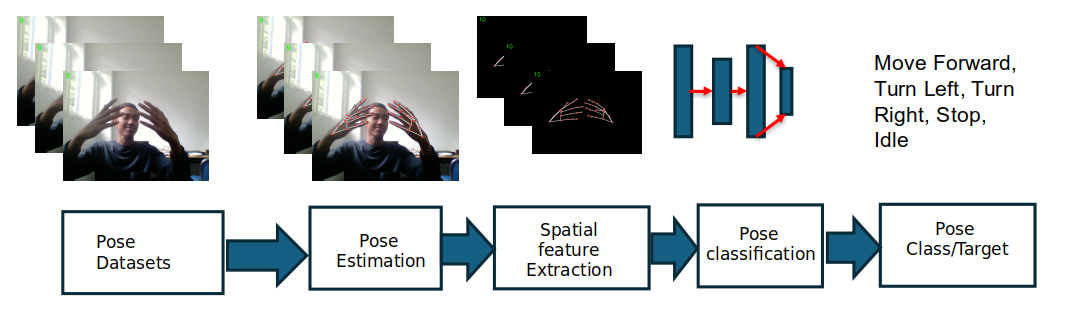
\includegraphics[width=\linewidth]{img/pose_pipeline} % Adjust the width or other parameters as needed
	\caption{Hand Recognition Pipeline}
	\label{fig:pose_pipeline} % Reference the figure in your text using \ref{fig:unique_label}
\end{figure}

\section{Dataset Acquisition}
This code provides a systematic way to acquire a dataset for hand pose recognition using Mediapipe and OpenCV. It captures hand landmarks and saves the corresponding frames from a webcam feed, enabling the creation of a labeled dataset for tasks like training gesture recognition models.

The process begins with the initialization and setup of necessary components. Mediapipe's Hands model is used for detecting and tracking hand landmarks, while OpenCV handles video capture and frame display. Command-line arguments allow customization of parameters such as the dataset path, label name, frame saving rate, maximum frames to save, and a delay before data collection starts. The script ensures that a directory for the dataset is created, organizing the captured data based on the provided label name. The Figure \ref{fig:data_acquisition} shows the sample of data acquisition.

\begin{figure}[h]
	\centering
	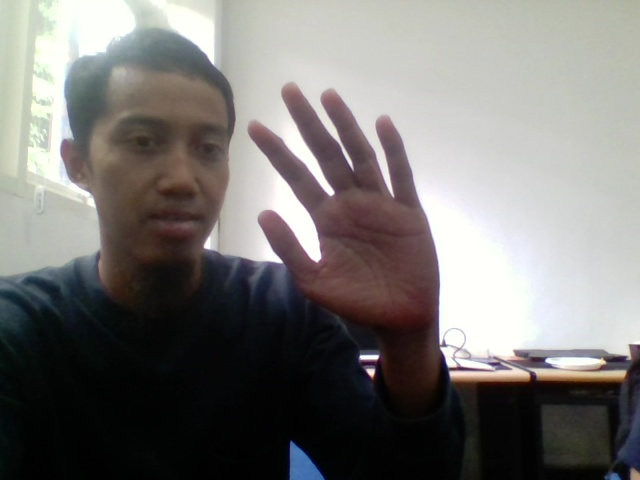
\includegraphics[width=0.3\linewidth]{img/data_cap1} 
	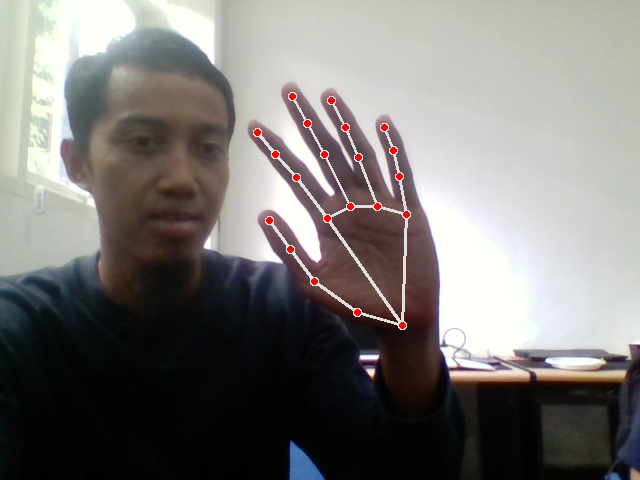
\includegraphics[width=0.3\linewidth]{img/data_cap2}
	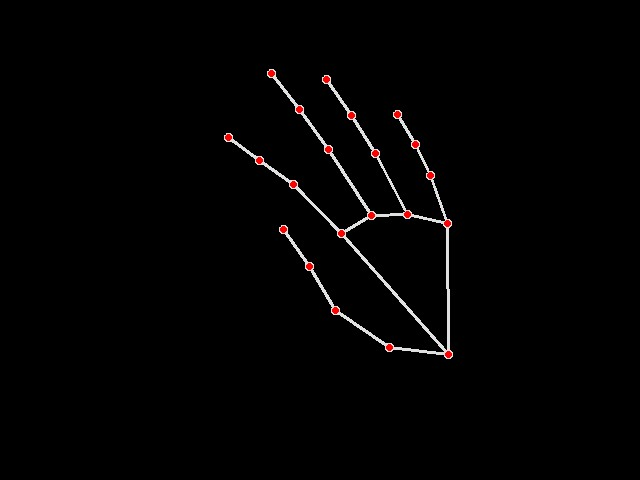
\includegraphics[width=0.3\linewidth]{img/data_cap3}
	\caption{Sample of Data Acquisition Process}
	\label{fig:data_acquisition} % Reference the figure in your text using \ref{fig:unique_label}
\end{figure}

 Hand detection and landmark extraction are key steps in the process. The Mediapipe Hands model detects 21 landmarks on each hand, including knuckles and fingertips, and supports tracking up to two hands simultaneously. For every frame captured, the script converts it to RGB format and processes it using Mediapipe. Landmark coordinates are normalized relative to specific reference points, such as the wrist and a finger joint, making the data invariant to variations in hand size and position. The normalized landmarks for both hands are then concatenated into a single array, representing the frame’s hand pose data.

\section{Pose Estimation}

The `create\_dataset` function is a crucial part of the pose estimation process. It facilitates the acquisition of hand pose data by capturing frames from a webcam feed, extracting hand landmarks using Mediapipe's `Hands` solution, and organizing the data into labeled directories. This function serves as the foundation for building datasets tailored to pose estimation tasks, enabling further applications like gesture recognition and motion analysis.

Pose estimation involves detecting and interpreting key hand landmarks in real-time. The function initializes Mediapipe's `Hands` module, which is capable of identifying 21 specific landmarks on each hand, such as fingertips, joints, and the wrist. These landmarks represent the structural configuration of the hand and are essential for understanding its pose. By converting the captured video frames to RGB format and processing them through Mediapipe, the function extracts these landmarks with high precision.

To normalize the landmark data, the function computes positions relative to key reference points—namely, the wrist and a finger joint. This normalization step ensures that the data remains invariant to hand size and camera perspective, enhancing its generalizability for machine learning models. The landmark coordinates for both hands are flattened into a single array, representing the spatial configuration of the hands in each frame.

Beyond pose estimation, the `create\_dataset` function also incorporates real-time feedback and organization. Frames are captured and saved at user-defined intervals, allowing control over the frame rate and total number of frames collected. Each frame is stored in a labeled directory, organized by the name of the gesture or pose being recorded. The overlay of the detected landmarks on the video feed, along with a live counter of saved frames, enhances the usability of the function by providing visual confirmation and progress tracking.

This function exemplifies the integration of pose estimation techniques with practical data collection workflows. It not only extracts meaningful pose information but also structures the data in a format ready for subsequent analysis and model training. This makes it a powerful tool for researchers and developers working on applications in gesture recognition, human-computer interaction, and beyond.

\subsection{Import required Python libraries}
\begin{lstlisting}
import cv2
import mediapipe as mp
import numpy as np
from datetime import datetime
import os
import time
import argparse
\end{lstlisting}

\subsection{MediaPipe Initialization}
\begin{lstlisting}
mp_hands = mp.solutions.hands
hands = mp_hands.Hands(static_image_mode=False,
max_num_hands=2,
min_detection_confidence=0.5,
min_tracking_confidence=0.5)

\end{lstlisting}

This part initializes the Mediapipe Hands solution, which is responsible for detecting hand landmarks in video frames. The configuration allows real-time processing of up to two hands per frame, with parameters controlling the confidence thresholds for detection and tracking. This setup ensures accurate and stable landmark recognition during data collection.

\subsection{ Webcam Access and Directory Setup}

\begin{lstlisting}
cap = cv2.VideoCapture(0)
save_dir = os.path.join(direktori_path, nama_label)
if not os.path.exists(save_dir):
	os.makedirs(save_dir)
	
\end{lstlisting}

The webcam is opened using OpenCV’s VideoCapture, which serves as the data source for real-time frame capture. The save\_dir is created dynamically based on the dataset path and label name, ensuring an organized directory structure for storing the collected data.

\subsection{Landmark Extraction}
\begin{lstlisting}
def ekstraksi_fitur(frame):
frame_rgb = cv2.cvtColor(frame, cv2.COLOR_BGR2RGB)
results = hands.process(frame_rgb)
height, width, _ = frame.shape
...
# Normalization and concatenation of landmarks
return np.concatenate((left_hand_landmarks.flatten(), right_hand_landmarks.flatten()))

\end{lstlisting}

This function extracts and processes hand landmarks from each frame:
\begin{enumerate}
	\item Conversion to RGB: Mediapipe requires frames in RGB format for processing.
	\item Landmark Processing: If hand landmarks are detected, their coordinates are normalized relative to reference points (e.g., the wrist and a finger joint) to ensure invariance to hand size and position.
	\item Concatenation: The landmarks for both hands are flattened and concatenated into a single array, representing the full pose information for the frame.
\end{enumerate}

\section{Geometric Feature Extraction}

\subsection{Function Definition and Initialization}
\begin{lstlisting}
def create_dataset(direktori_path, nama_label, frameratesave=2, maxframe=100, start_delay=5):
	
	# Initialize Mediapipe Hands and Drawing
	mp_hands = mp.solutions.hands
	mp_drawing = mp.solutions.drawing_utils
	hands = mp_hands.Hands(static_image_mode=False,
	max_num_hands=2,
	min_detection_confidence=0.5,
	min_tracking_confidence=0.5)
	
\end{lstlisting}
The create\_dataset function begins with its definition, which includes several customizable parameters: the dataset directory (direktori\_path), the label for the dataset (nama\_label), the frame saving rate (frameratesave), the maximum number of frames to save (maxframe), and the delay before starting the capture (start\_delay). Inside the function, the Mediapipe Hands model is initialized. This model is set up to dynamically process video streams (static\_image\_mode=False) and detect up to two hands simultaneously. Detection and tracking confidence thresholds are set to 0.5, balancing accuracy and performance. The DrawingUtils module is also initialized for later use in visualizing detected landmarks.
\subsection{Webcam Initialization and Directory Setup}
\begin{lstlisting}
	    # Open webcam
	cap = cv2.VideoCapture(0)
	if not cap.isOpened():
	     print("Failed to open webcam.")
	     return
	
	# Create directory path
	save_dir = os.path.join(direktori_path, nama_label)
	if not os.path.exists(save_dir):
	     os.makedirs(save_dir)
	     print(f"Directory created: {save_dir}")
	
\end{lstlisting}
Next, the function initializes the webcam using OpenCV’s VideoCapture. If the webcam cannot be opened, an error message is printed, and the function exits gracefully. The function then prepares the directory for storing the dataset. If the directory does not already exist, it is created using os.makedirs. The dataset is organized by the label provided (nama\_label), ensuring clear structure and traceability for the saved frames.

\subsection{Countdown Timer and Frame Processing}
Before data collection begins, the function sets up a countdown timer \verb|start_delay| using \verb|time.time()|. The \verb|ekstraksi_fitur| function processes each frame. It converts the frame to RGB (as required by Mediapipe) and detects hand landmarks using the \verb|hands.process| method. If landmarks are detected, they are normalized relative to specific reference points (e.g., the wrist and a finger joint) to account for hand size and positioning. The normalized coordinates for the left and right hands are stored in separate arrays and concatenated for a unified representation.\\

\begin{lstlisting}
	
time_before = datetime.now()
start_time = time.time()
counter = 0
	
def ekstraksi_fitur(frame):
	# Convert to RGB
	frame_rgb = cv2.cvtColor(frame, cv2.COLOR_BGR2RGB)
	
	# Process frame with Mediapipe
	results = hands.process(frame_rgb)
	
	# Frame dimensions
	height, width, _ = frame.shape
	
	# Initialize numpy arrays for left and right hands
	left_hand_landmarks = np.zeros((21, 2))
	right_hand_landmarks = np.zeros((21, 2))
	
	# Helper function to process landmarks
	def process_landmarks(hand_landmarks, width, height):
		landmarks = [(lm.x * width, lm.y * height) for lm in hand_landmarks.landmark]
		landmark_0 = np.array(landmarks[0])
		landmark_5 = np.array(landmarks[5])
		normalized_landmarks = [
			((x - landmark_0[0]) / (landmark_5[0] - landmark_0[0] + 1e-6),
			(y - landmark_0[1]) / (landmark_5[1] - landmark_0[1] + 1e-6))
			for x, y in landmarks
		]
	return np.array(normalized_landmarks)
	
	# If hands are detected
	if results.multi_hand_landmarks and results.multi_handedness:
		for hand_landmarks, hand_handedness in zip(results.multi_hand_landmarks, results.multi_handedness):
		# Identify hand as left or right
		handedness = hand_handedness.classification[0].label
		processed_landmarks = process_landmarks(hand_landmarks, width, height)
		if handedness == 'Left':
			left_hand_landmarks = processed_landmarks
		elif handedness == 'Right':
			right_hand_landmarks = processed_landmarks
		
		# Draw landmarks on the frame
		mp_drawing.draw_landmarks(frame, hand_landmarks, mp_hands.HAND_CONNECTIONS)
		
		# Concatenate left and right hand landmarks
	concatenated_landmarks = np.concatenate((left_hand_landmarks.flatten(), right_hand_landmarks.flatten()))
	return concatenated_landmarks
\end{lstlisting}

\subsection{Frame Capture and Saving}
\begin{lstlisting}
while cap.isOpened():
	ret, frame = cap.read()
	if not ret:
		print("Failed to read frame from webcam")
		break
	
	# Countdown before saving starts
	elapsed_time = time.time() - start_time
	if elapsed_time < start_delay:
		countdown_text = f"Starting in {int(start_delay - elapsed_time)} seconds"
		cv2.putText(frame, countdown_text, (10, 50), cv2.FONT_HERSHEY_SIMPLEX, 1, (0, 0, 255), 2)
		cv2.imshow('Hand Landmark Detection', frame)
		if cv2.waitKey(1) & 0xFF == ord('q'):
			break
		continue
	
	# Check framerate and save frame
	time_now = datetime.now()
	if (time_now - time_before).total_seconds() > 1 / frameratesave:
		# Generate file name
		file_name = datetime.now().strftime("%Y%m%d%H%M%S%f")[:-3] + ".jpg"
		file_path = os.path.join(save_dir, file_name)
		
		# Save frame
		cv2.imwrite(file_path, frame)
		counter += 1
	
		# Update the previous time
		time_before = time_now
	
	# Display counter on frame
	cv2.putText(frame, f"Files saved: {counter}", (10, 50), cv2.FONT_HERSHEY_SIMPLEX, 1, (0, 255, 0), 2)
	
	# Process landmarks and draw them on the frame
	concatenated_landmarks = ekstraksi_fitur(frame)
	print("Concatenated Landmarks:", concatenated_landmarks)
	
	# Display the frame with landmarks
	cv2.imshow('Hand Landmark Detection', frame)
	
	# Stop saving after maxframe is reached
	if counter >= maxframe:
		print(f"Reached maximum of {maxframe} frames. Exiting...")
		break
	
	# Handle key press
	key = cv2.waitKey(1) & 0xFF
	if key == ord('q'):  # Exit on 'q'
		break
	

\end{lstlisting}

The webcam feed is processed frame by frame. During the countdown period, a message informs the user of the time remaining before data collection begins. Once the countdown ends, frames are saved at intervals defined by the \verb|frameratesave| parameter. Each frame is assigned a timestamp-based filename and stored in the appropriate directory. The landmarks are processed in real-time, printed to the console, and visualized on the webcam feed using Mediapipe’s drawing utilities.

\subsection{Cleanup}
\begin{lstlisting}
	# Release resources
	cap.release()
	cv2.destroyAllWindows()
	hands.close()
\end{lstlisting}
After reaching the specified frame limit or upon user interruption, the function releases the webcam and closes all OpenCV windows. The Mediapipe Hands object is also closed, ensuring that all resources are properly deallocated. This function effectively combines pose estimation, real-time feedback, and dataset organization, making it a comprehensive tool for collecting hand pose data.
\section{Model Architecture}

\begin{figure}[h]
	\centering
	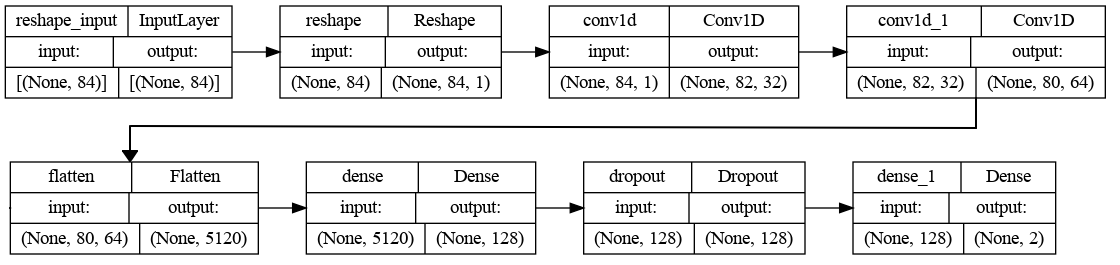
\includegraphics[width=\linewidth]{img/model_architecture} % Adjust the width or other parameters as needed
	\caption{Model Architecture}
	\label{fig:model_architecture} % Reference the figure in your text using \ref{fig:unique_label}
\end{figure}

This model represents a simple feed-forward neural network designed for tasks such as classification, particularly for hand pose recognition. The architecture utilizes Convolutional Neural Network (CNN) model implemented in TensorFlow, specifically designed for tasks involving 1D data, such as time-series analysis, signal processing, or structured data (like hand pose landmarks).

\begin{lstlisting}
	Reshape((input_size, 1), input_shape=(input_size,))
\end{lstlisting}

This layer reshapes the 1D input vector of size \verb|(input_size,)| into a 2D array with dimensions \verb|(input_size, 1)|. This transformation is necessary because Conv1D layers require a 2D input format where one dimension represents the sequence length \verb|(input_size)|, and the other represents the number of channels (here, a single channel).

The reshaped input is then passed to the first Conv1D layer:
\begin{lstlisting}
	Conv1D(filters=32, kernel_size=3, activation='relu')
\end{lstlisting}

This layer applies 32 convolutional filters with a kernel size of 3 to extract local patterns from the data. The \verb|relu| activation introduces non-linearity, enabling the model to learn complex features. The next layer is another Conv1D layer:
\begin{lstlisting}
	Conv1D(filters=64, kernel_size=3, activation='relu')
\end{lstlisting}
This layer increases the number of filters to 64, allowing it to capture more complex patterns and higher-level features from the output of the previous layer. Both convolutional layers reduce the dimensions of the input while retaining its essential features.

After the convolutional layers, a Flatten layer:
\begin{lstlisting}
	Flatten()
\end{lstlisting}
is used to convert the multi-dimensional output from the Conv1D layers into a 1D vector. For example, if the output from the second Conv1D layer is of shape (80, 64), the Flatten layer transforms it into a vector of size (80 * 64 = 5120). This step prepares the data for the subsequent fully connected layers.

The flattened output is fed into a Dense layer:
\begin{lstlisting}
	Dense(128, activation='relu')
\end{lstlisting}

which consists of 128 neurons. Each neuron applies a linear transformation followed by a \verb|relu| activation function to learn combinations of features extracted by the convolutional layers. This dense layer reduces the feature space while focusing on the most significant patterns.

To prevent overfitting, the model includes a Dropout layer:
\begin{lstlisting}
	Dropout(0.5)
\end{lstlisting}
which randomly deactivates 50\% of the neurons during training. This regularization technique ensures that the model does not rely too heavily on specific neurons, improving its ability to generalize to unseen data.

Finally, the model ends with an output Dense layer:
\begin{lstlisting}
	Dense(num_classes, activation='softmax')
\end{lstlisting}
This layer has a number of neurons equal to the number of target classes (\verb|num_classes|). The \verb|softmax| activation function converts the raw outputs into probabilities for each class, ensuring that the sum of all probabilities equals 1. This makes it suitable for multi-class classification tasks.

Overall, the model starts with reshaping the input, extracts meaningful features using convolutional layers, flattens the extracted features, and uses dense layers for classification, with dropout for regularization. The final softmax layer outputs class probabilities, making it effective for tasks like hand pose classification or time-series analysis.
\section{Pose Classification}
\section{Pose Inference}